\section*{Лекція 2: Математика в Python}

\subsection{Змінні}
 
\begin{frame}
\frametitle{Дані в Python}
\begin{itemize}
  \item Змінна - посилання на об'єкт
  \item Оператор присвоювання: 
  
  \texttt{Операнд зліва = Операнд зправа}
  \item Динамічна типізація
  \item \texttt{a = 7; b = a}
  \item Каскадне присвоювання: \texttt{a = b = c = 0}
  \item Множинне присвоювання: \texttt{a, b = 1, 2}
  \item Обмін значеннями: \texttt{a, b = b, a}
\end{itemize}
\end{frame}

\begin{frame}
\frametitle{Функція id}
Функція id(object) повертає «ідентифікаційний номер» об'єкта object, який є унікальним та незмінним.
\begin{figure}
\begin{center}
 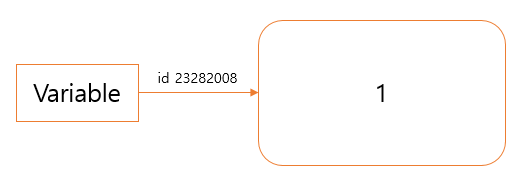
\includegraphics[width=0.7\textwidth]{pictures/id_func.png}
\caption{Функція id}
\label{id} 
\end{center}
\end{figure}
\end{frame}

\begin{frame}
\frametitle{Функція type}
type(object) повертає тип об'єкту object (object .\_\_ class\_\_).
\begin{figure}
\begin{center}
 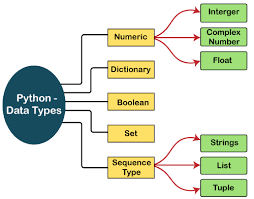
\includegraphics[width=0.5\textwidth]{pictures/python_data_types.png}
\caption{Типи даних в Python}
\label{data_types} 
\end{center}
\end{figure}
\end{frame}


\begin{frame}
\frametitle{Імена змінних}
\begin{itemize}
  \item Перший символ - будь-яка літера латинського алфавіту a-z, A-Z та символ підкреслення \_. Інші символи - теж саме та цифри 0-9.
  \item Іменами слід обирати іменники.
  \item Імена повинні відображати сенс даних.
  \item Неможна використовувати зарезервовані слова (Pycharm - Python Console - help() - keywords).
  \item Не слід використовувати імена вбудованих функцій.
\end{itemize}
\end{frame}

\subsection{Числа}
 
\begin{frame}
\frametitle{Типи чисел в Python}
\begin{itemize}
  \item цілі числа (int);
  \item дійсні числа (float);
  \item комплексні числа (complex).
\end{itemize} 
  
\end{frame}

\begin{frame}
\frametitle{Експоненційне представлення чисел}
Python підтримує експоненційне представлення чисел. Наприклад:

\LARGE{
$5e2 = 5\ast 10^2 = 5\ast 100 = 500$

$1e-2 = 1\ast 10^{-2} = 1\ast 0.01 = 0.01$  
}
\end{frame}

\begin{frame}
\frametitle{Cистеми числення}
У Python можна використовувати різні системи числення. 
\begin{itemize}
\item Запис двійкового числа розпочинається з \texttt{0b}.
\item Щоб представити число в двійковій формі використовується функція \texttt{bin}.
\item Запис шістнадцяткового числа розпочинається з \texttt{0x}.
\item Запис вісімкового числа розпочинається з \texttt{0o}. 
\end{itemize}
\end{frame}


 
\begin{frame}
\frametitle{Арифметичні операції}

\begin{table}
  \caption{Арифметичні операції}
  \label{tab:}

  \begin{center}
    \begin{tabular}{|c|c|c|}
      \hline
      \textbf{Оператор} & \textbf{Опис} & \textbf{Пріоритет} \\
      \hline
      +, - & додавання, віднімання & 2 \\
       \hline
      * & множення & 3 \\
       \hline
       /,// & ділення & 3 \\
       \hline
       \% & залишок від ділення & 3 \\
       \hline
       ** & піднесення в ступінь & 4 \\
       \hline
    \end{tabular}
  \end{center}
\end{table}
 \begin{center}
   \tiny{// - ділення з округленням до найменшого цілого}
  \end{center}
\end{frame}

\begin{frame}
\frametitle{Скорочені оператори в Python}
\begin{table}
  \caption{Скорочені арифметичні оператори}
  \label{tab:}

  \begin{center}
    \begin{tabular}{|c|c|}
      \hline
      \textbf{Операція} & \textbf{Скорочений запис} \\
      \hline
      i = i + 1 & i += 1 \\
       \hline
      i = i - 1 & i -= 1 \\
       \hline
      i = i*2 & i *= 2  \\
       \hline
      i = i/2 & i /= 2 \\
       \hline
      i = i//2 & i //= 2 \\
       \hline
      i = i\%2  & i \%= 2 \\
       \hline
      i = i**2 & i **= 2 \\
       \hline
    \end{tabular}
  \end{center}
\end{table}
\end{frame}

\subsection{Математичні операції}

\begin{frame}
\frametitle{Математичні функції}
\begin{itemize}
  \item abs(a)
  \item min(a, b, ...)
  \item max(a, b, ...)
  \item pow(a, b)
  \item round(a)
  \item round(a, n)
\end{itemize} 
  
\end{frame}

\begin{frame}
\frametitle{Модуль math}
Для того щоб звернутися до функцій модулю math, спочатку треба імпортувати цей модуль командою \texttt{import math}.
\begin{figure}
\begin{center}
 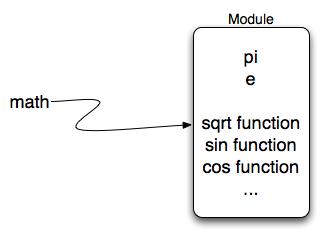
\includegraphics[width=0.5\textwidth]{pictures/mathmod.png}
\caption{Модуль math}
\label{mathmodule} 
\end{center}
\end{figure}
\end{frame}

\subsection{Вивід та ввід інформації}

\begin{frame}
\frametitle{Функції print та input}
\begin{itemize}
  \item print - вивід даних в консоль
      \begin{itemize}
        \item sep - роздільник між даними
        \item end - останній символ (символи)
     \end{itemize} 
  \item input - ввід даних зі стандартного вхідного потоку (клавіатури)
      \begin{itemize}
        \item int(input())
        \item float(input())
     \end{itemize}
 \end{itemize} 
\end{frame}
